
\documentclass[preprint,12pt]{elsarticle}

\usepackage[spanish]{babel}
\usepackage{amssymb}
\usepackage{graphicx}
\usepackage{lineno}
\usepackage[utf8]{inputenc}
\usepackage{url}
\usepackage{color}
\usepackage{enumerate} 
\usepackage[hidelinks]{hyperref}


\begin{document}
	
	\begin{frontmatter}
		
		
		\title{\huge Dimensional vs Modelo Tabular}
		
		\author{Mamani Ayala, Brandon        (2015052715)}
		\author{Quispe Mamani, Angelo	      (2015052826)}
		\author{Vizcarra Llanque, Jhordy	      (2015052719)}
		\author{Ordoñez Quilli, Ronald          (2015052821)}
		\author{Rodriguez Mamani, Juan      (2017057862)}
		
		\address{Tacna, Perú}
		
		\begin{abstract}
			%% Text of abstract
			
The data warehouses in English take each importance day, as organizations move from schemes of only data collection to schemes of analysis of the same. However, in spite of the great diffusion of the concepts related to data warehouses, there is not too much Information available in Spanish regarding the methodologies fo implement them In this short article we will try to provide a general explanation of one of the most used methodologies. 
		\end{abstract}
\end{frontmatter}
%%

	
	%%
	%\linenumbers
	
	%% main text
	\section{Resumen}
Los almacenes de datos (data warehouses en inglés) toman cada día mayor importancia, a medida que las organizaciones pasan de esquemas de sólo recolección de datos a esquemas de análisis de los mismos. Sin embargo a pesar de la gran difusión de los conceptos relacionados con los almacenes de datos, no existe demasiada información disponible en castellano en cuanto a las metodologías para implementarlos. En este breve artículo intentaremos brindar una explicación general de una de las metodologías más usadas \\
	%%
	
	%%
	%\linenumbers
	
	%% main text



	%%
	
	%%
	%\linenumbers
	
	%% main text

\section{Marco Teorico}
\subsection{Modelo Dimensional}
El modelo de datos dimensional proporciona un método para simplificar y facilitar la comprensión de las bases de datos. Una base de datos dimensional se puede concebir como un cubo de tres o cuatro dimensiones en el que los usuarios pueden acceder a una porción de la base de datos a lo largo de cualquiera de sus dimensiones.\\

Para crear una base de datos dimensional, necesita un modelo que le permita visualizar los datos.\\
\begin{center}
	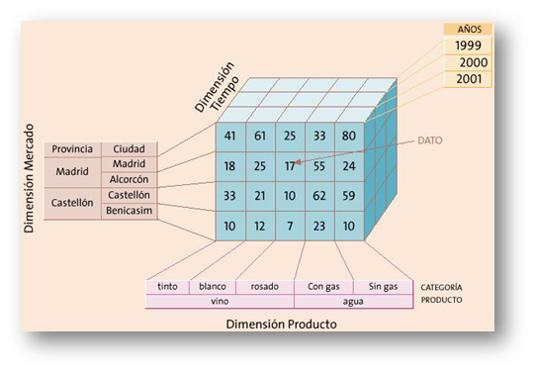
\includegraphics[width=14cm]{./Imagenes/jho1} 
\end{center}
Otro nombre que se utiliza para el modelo dimensional es esquema de estrella-unión. Los diseñadores de bases de datos utilizan este nombre porque el diagrama de este modelo parece una estrella con una tabla central alrededor de la cual se muestran un conjunto de otras tablas.\\

La tabla central es la única tabla del esquema con varias uniones que la conectan con todas las demás tablas. Esta tabla central se denomina la tabla de hechos y las demás tablas se denominan tablas de dimensiones.\\

Todas las tablas de dimensiones tienen una sola unión que las conecta con la tabla de hechos, independientemente de la consulta.\\
\begin{center}
	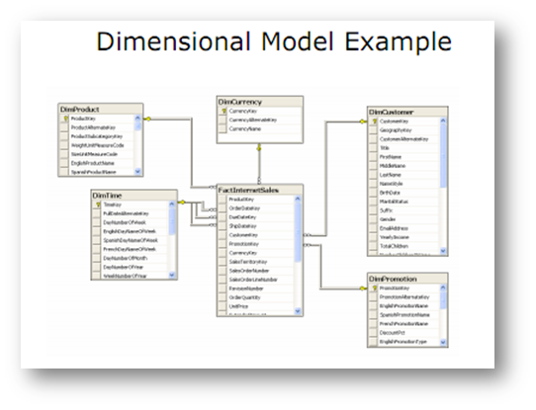
\includegraphics[width=14cm]{./Imagenes/jho2} 
\end{center}

\subsection{Desarrollo de Modelo Tabular}

Los encargados de tomar decisiones  reconocen que  hoy día  es imposible  actuar basándose  solo en  la intuición para hacer crecer su negocio o para permanecer exitosamente en el mercado. Vinculado a esta premisa, ha evolucionado un conjunto de conceptos, modelos y tecnologías con el transcurso de los años cuya interacción facilita la acertada conducción de cualquier negocio.  La Inteligencia de Negocios (BI, del inglés Business Intelligence) se puede definir como un conjunto de metodologías,  procesos,  arquitecturas  y  tecnologías  que  transforman  datos  en  información  útil  e importante que posibilita ideas estratégicas, tácticas y operativas más eficaces para la toma de decisiones .\\
\\
Se materializa cuando se proveen herramientas y políticas organizacionales a nivel empresarial que permiten a los directivos transformar la  información clave  de su empresa en acciones concretas que se traduzcan  en  beneficios  palpables.  Hoy  se  ha  convertido  en  un  modelo  de  control  y  crecimiento corporativo para lograr competitividad. Una frase popular acerca de la Inteligencia de Negocios plantea: “Inteligencia de Negocios es el proceso de convertir datos en conocimiento y el conocimiento en acción para la toma de decisiones” .\\
\\
Las  exigencias  actuales del  mercado  están  conduciendo  a que  las  empresas  incorporen  a  su  gestión soluciones integrales de BI que cubran las necesidades informacionales de sus ejecutivos, para hacerlas crecer  de manera  competitiva. En realidad, resulta  más  pertinente hablar  de sistemas  o soluciones  de Inteligencia de Negocios como aproximaciones sucesivas, puesto que no existe un modelo único para su desarrollo, dado el alcance y  la complejidad  del proceso [8]. En este sentido,  numerosas compañías de software  han  producido  plataformas  que  integran  varias  herramientas,  ofreciendo  a  las  empresas  un producto completo que responda a las diferentes etapas del proceso de BI, a partir del cual los equipos de desarrollo  pueden  generar  con  mayor  holgura  y  productividad  las  aproximaciones  de  soluciones  BI propias. La  plataforma de  Inteligencia de  Negocios de Microsoft  ha sido  seleccionada para la presente investigación por las facilidades que posee, su utilización en innumerables soluciones computacionales a nivel mundial  y en  CIMEX como caso  particular, donde se  cuenta con  más de 8  años de  experiencias usando este tipo de plataformas.\\
\\
A partir de la versión SQL Server 2012 Analysis Services (Tabular), el motor de búsquedas Vertipaq fue renombrado como el motor de búsqueda analítico en memoria xVelocity (del inglés, xVelocity in-memory analytics engine), el cual logró un cambio sustancial en el rendimiento de las consultas analíticas debido a la  utilización  de  técnicas  tales  como almacenamiento  por  columnas,  compresión  de  datos,  caché  en memoria  y  algoritmos  de  escaneo  y  agregación  de  datos  en  paralelo . \\
\\
El  almacenamiento  por columnas significa que cada página de datos contiene valores de una sola columna, además, en el proceso de indización se conservan los valores repetidos solo una vez y se sustituyen las cadenas de texto y fechas por números enteros, todo  lo cual  favorece la  compresión de  los datos  . Se  plantea que  la tasa  de compresión de datos está en el orden de 10:1 - 15:1 y cuando hay muchos valores repetidos puede ser de 1000:1. Por otra parte, las bases de datos in-memory utilizan la memoria principal de la máquina (RAM, del inglés  Random Access  Memory) para el almacenamiento  de los datos. Desde  el punto de vista  del usuario final, xVelocity posibilita rápidos accesos a los datos almacenados en las bases de datos tabulares utilizando  las aplicaciones  clientes como  Excel y  Power View,  lo cual se  considera  una  mejora  en el rendimiento  de  las  consultas  de  entre  10  y  100  veces  .  Power  View  constituye  una  intuitiva herramienta de reportes en la que los usuarios pueden interactuar con las vistas de su negocio publicadas en Analysis Services, cualquiera sea el modelo analítico .



\subsection{Los Modelos multidimensional y tabular en la solucion BI}

La actividad  comercial de  CIMEX con  alcance nacional  y su  extensa red  minoristas con  más de 900 tiendas constituye uno de los baluartes de este grupo empresarial y genera diariamente un gran volumen de datos. Por tal motivo, resulta imprescindible mantener el control de los procesos principales que tienen lugar  en  cada  uno  de los  establecimientos  con  el  objetivo  de  brindar información  actualizada  a  los analistas y directivos de la corporación, así como a otras entidades del país. En el escenario comercial se realizan varias operaciones que provocan movimientos de entrada y salida en el inventario relacionadas con  los  conceptos  compra  y  venta  de  mercancías,  transferencias  y  ajustes,  cuyo comportamiento  se analiza a partir de un conjunto de indicadores comerciales.   Actualmente  se  cuenta  con  un  sistema  de  gestión  de  información  que  incluye  almacenes  de  datos operacionales (ODS, del inglés Operational Data Store) como repositorio de datos, con detalle diario y frecuente actualización, mediante el cual se logran tener los datos de manera centralizada y consolidada, brindando a los usuarios nuevas funcionalidades y el acceso web a la misma información desde cualquier establecimiento. Los reportes,  ya sean comerciales o contables,  aún se encuentran sujetos a esquemas predefinidos con posibilidades limitadas de navegación.  Adicionalmente, se  cuenta con  un portal  web para  el apoyo  a la  toma  de decisiones,  denominado Sistema  de Administración  de Negocios  (SAN), desarrollado desde el año 2008. SAN muestra reportes estáticos sobre diferentes procesos de negocio que se interrelacionan, brindando a los directivos un conjunto de aplicaciones que abarcan desde la etapa de planificación  y  ejecución de  los  procesos hasta  la evaluación  mediante  indicadores  comerciales  y  la emisión automática de boletines.  La mayoría de las aplicaciones desarrolladas responde directamente a los procesos del negocio y no a los sujetos  de análisis.  Hasta el  momento no  había  sido  posible integrar  las informaciones  comerciales y contables, así como de  otras áreas,  ni comprobar  el grado de correspondencia entre  ellas con  vistas a evaluar  el  funcionamiento  de  la  organización.\\
\\
Tampoco  se  garantizaba  la información  histórica  que permitiera realizar análisis retrospectivos ni perspectivos que contemplaran las transformaciones efectivas y posibles en el transcurso del tiempo durante la toma de decisiones. Esta problemática se estudió en la investigación desarrollada,  la cual  se orientó  a la  concepción, diseño e implementación  de una  nueva aproximación de solución de Inteligencia de Negocios que permita el análisis informacional integrando los datos de diferentes áreas de CIMEX, valorando las contribuciones y los inconvenientes del empleo de los modelos multidimensional y tabular al respecto. Una de las principales tareas en el desarrollo de esta solución fue identificar los requerimientos informacionales, a partir de entrevistas e intercambios con los usuarios analistas.  Desde el punto de vista informacional, la propuesta de solución de Inteligencia de Negocios se centra en el diseño  e implementación de un  almacén de datos orientado al  análisis, que  contiene la información comercial y contable de CIMEX. El ambiente web desarrollado sobre SharePoint existente en la empresa se usa para la presentación de los resultados, proporcionando además la navegación por los escenarios de análisis, la confección dinámica de consultas y el enriquecimiento de los efectos visuales. En la Fig. 1 se muestra el modelo general de la solución propuesta.



\begin{center}
	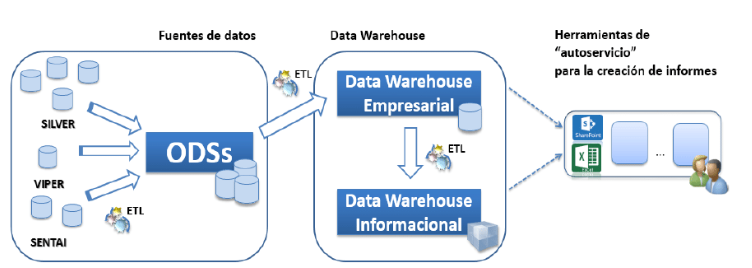
\includegraphics[width=12cm]{./Imagenes/ang2} 
\end{center}

El almacén de datos se basa en la arquitectura de datos de tres capas propuesta por Devlin  y también conocida como Enterprise data warehouse . Se identifican como componentes fundamentales: el data warehouse empresarial, el data warehouse informacional y la presentación de la información. Cabe apuntar que, aun cuando las  fuentes constituyen almacenes de datos operacionales con sus procesos  de carga respectivos, el  diseño y la  instrumentación del  proceso de población del  data warehouse se  han caracterizado  por  un  examen  minucioso  de  los  datos  disponibles  en  función  de  la  calidad  de  la información suministrada para la toma de decisiones.  \\ 
\\
La primera capa de datos corresponde a las  fuentes de  datos que poseen información de los  procesos contables y comerciales relacionados con el comercio minorista en CIMEX, que constituyen almacenes de datos operacionales (ODS) provenientes de los sistemas transaccionales.  La segunda capa o capa de datos conciliados corresponde al data warehouse empresarial (DWE), el cual constituye un repositorio único que concilia la  información contable  y comercial disponiendo los datos para el análisis. El data warehouse empresarial es una base de datos relacional en Tercera Forma Normal preparada para almacenar la información histórica.  La tercera capa o capa de datos derivados corresponde al  warehouse informacional (WI), que posee un diseño  orientado  a apoyar  la  toma de  decisiones  de  modo  que los  datos  previamente  conciliados  se denormalizan y agrupan con el fin de garantizar buenos tiempos de respuestas durante la navegación y las consultas informacionales.  \\ 
\\
La  solución posee  además una  capa final  de presentación  de la  información que  proporciona  mayor dinamismo a partir de la experiencia interactiva con los datos. En esta capa se utilizan herramientas como Power View  sobre SharePoint y las  tablas dinámicas  de Excel, poniendo a  disposición de los  usuarios funcionalidades de autoservicio, tanto para la navegación como para la creación de nuevas consultas.  En  el  diseño  informacional  del  repositorio  de  datos  se  concibió  la  creación  de  estructuras multidimensionales  que  responden a  los requerimientos  generales. Los  sujetos del  negocio  modelados dentro del escenario comercial son: Ventas, Compras, Inventario, Transferencias, Ajustes y Vales. En el escenario contable se modeló el Mayor General, las Cuentas por Cobrar y las  Cuentas por Pagar.  La integración de  estos procesos  de negocios se  lleva a  cabo a  partir del diseño del esquema dimensional “Validación de Ventas” y se concibió el cubo virtual “Análisis Comercial y Contable”.  

\begin{center}
	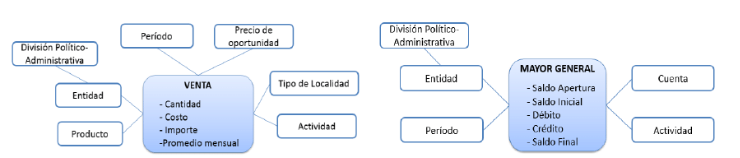
\includegraphics[width=12cm]{./Imagenes/ang3} 
\end{center}

La  población  del  warehouse  informacional  corresponde  a  la  implementación  de  las  bases  de  datos analíticas  en  SQL  Server  2012  Analysis  Services,  el  cual  propone  varias  alternativas  para  hacerlo, independientes entre sí, por lo que se debe decidir por una de ellas desde su instalación. En la solución propuesta se implementaron dos proyectos, uno utilizando el modelo multidimensional y otro, el modelo tabular. Asimismo, se preparó un conjunto de experimentos prácticos que validan y evalúan las variantes de solución.  \\ 
\\
En la herramienta SQL Server Data Tools se definieron las estructuras multidimensionales y tabulares que responden a los requerimientos informacionales realizados al inicio. La fuente de datos en ambos casos está constituida por el data warehouse empresarial. Algunas transformaciones fueron aplicadas al origen de datos como la creación de columnas calculadas, para lo cual se utiliza el lenguaje MDX en el modo multidimensional y el lenguaje DAX para el modo tabular. DAX (del inglés Data Analysis Expression) es el lenguaje de expresión de fórmulas analíticas que se utiliza para definir cálculos personalizados en los modelos  tabulares  y en  las  tablas  dinámicas de  Excel  a  través de  Power  Pivot.  Las  fórmulas  DAX incluyen  funciones,  operadores  y  valores  para  realizar  cálculos  avanzados  en  tablas  y  columnas relacionales. Estos dos lenguajes de consultas atienden a los diferentes conceptos de modelación, debido a que MDX tiene una semántica basada en dimensiones, atributos, jerarquías y medidas, mientras que DAX está basado en tablas y columnas.   \\
\\
Una vez definida la disposición de la fuente de datos, se instrumentaron las estructuras para el warehouse informacional según los esquemas dimensionales diseñados. En el modelo tradicional cada esquema se implementó  creando  cubos  multidimensionales  con las  medidas  y  las dimensiones  respectivas.  En  el modelo  tabular los  esquemas  se implementaron  mediante tablas  que  se relacionan  entre  sí para  fines analíticos. Ambos modelos no ofrecen las mismas funcionalidades, en la Tabla 1 se presenta un resumen de la disponibilidad de las características analíticas más relevantes de cada uno.

\begin{center}
	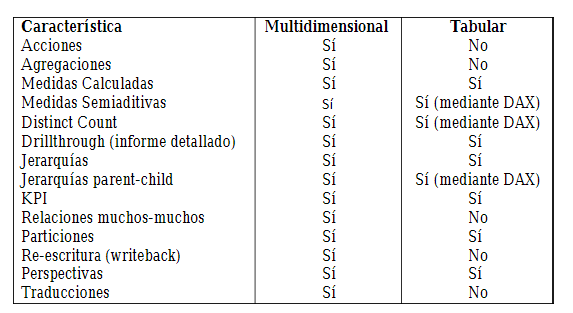
\includegraphics[width=12cm]{./Imagenes/ang4} 
\end{center}

El modelo dimensional utiliza el almacenamiento por filas, requiriéndose más recursos de lectura de disco y  menos  de  procesamiento  de  CPU.  Por  su  parte,  el  modelo  tabular  utiliza  el  almacenamiento  por columnas, de modo que el procesamiento de consultas requiere  más de la  utilización  de CPU  que de lectura a disco . Ambas soluciones utilizan compresión de datos dado que reducen el tamaño de las bases de datos de Analysis Services. Ahora bien, resulta crucial considerar que si los requerimientos de tamaño están en el orden de los terabytes, la solución tabular puede no ser conveniente si se tiene poca disponibilidad en memoria (RAM). Existen opciones de paginado para las soluciones tabulares, pero las grandes cantidades de datos se manejan mejor en soluciones multidimensionales. La Tabla 2 resume las características  esenciales de  los servidores de  Analysis Services  que se  deben tener en  cuenta para  la selección del modelo según los recursos disponibles . 

\begin{center}
	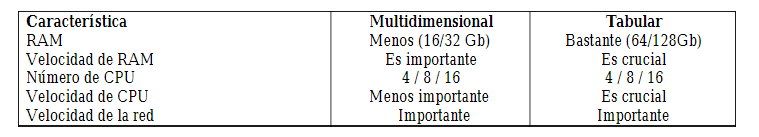
\includegraphics[width=12cm]{./Imagenes/ang5} 
\end{center}

\subsection{Experimentacion y valoraciones generales}

Con  el  propósito  de  validar  la  solución  propuesta,  se  diseñaron  cuatro  experimentos  que  permiten corroborar algunos de los supuestos teóricos a los cuales se ha arribado en la presente investigación. Los experimentos responden a las principales fases en la implementación y la presentación de los resultados. Debido al  gran volumen de datos existente en los sistemas  fuentes, correspondientes a  los últimos  tres años, en el escenario comercial se utilizaron los datos de tres de las principales sucursales de CIMEX en el país, a saber: Pinar del Río, Holguín y La Habana. En el escenario contable se emplearon los datos de todas las entidades de CIMEX.  Los experimentos  diseñados se  ejecutaron en  un servidor  con sistema operativo  Windows  Server  2008  R2  Standard  (Service  Pack  1),  un  procesador  Dual-Core  AMD Opteron(tm) Processor 2218 de velocidad 2.60 GHz, con memoria RAM de 3.00 GB y una arquitectura de 64 bit.  \\
\\
El primer experimento corresponde a la población del DWE y se concibió con el objetivo de comprobar la capacidad de los procesos ETCL implementados para poblar la capa de datos conciliados, destacando que es independiente de los modelos multidimensional y tabular. Para analizar los tiempos de ejecución de la carga  inicial  y  posterior  actualización,  se  dividió  el  experimento  en  tres  fases.  La  primera  de  ellas corresponde a la población de los criterios de análisis; luego se cargaron los datos de las Compras de los últimos tres  años, brindando una idea  del tiempo de  la carga inicial para  un sujeto de análisis y en  la última fase se ejecutaron todos los procesos ETCL para  un mes, que es el período de actualización del DWE.  Como  resultado de  este  primer experimento,  se  comprobó  que  los procesos  ETCL  funcionan correctamente. Se cargaron 1.2 millones de registros de dimensiones en 40 min. y 830 mil registros de hechos de un mes (marzo/2013) en 42 min., ocupándose finalmente un espacio de 2.6 Gb. El tiempo de ejecución  en  este  experimento  se  considera  aceptable,  dado  el  volumen  de  datos  manejados  y  el procesamiento necesario para garantizar tanto la integridad referencial como la integración real de ambos escenarios.  \\ 
\\
El segundo experimento corresponde a la población de la capa de datos derivados y se concibió con el objetivo  de  analizar  el  comportamiento  del  proceso  de  población  del  WI  para  los  dos  modelos implementados, así como comparar los resultados obtenidos en cada caso. Para ello, se consideraron dos fases,  correspondientes  a  la  población  de  cada  una  de  las  bases  de  datos  analíticas  de  la  solución implementada para  un mes  (marzo/2013). Pudo concluirse que el modelo  tabular es  más rápido que el modelo multidimensional en cuanto a tiempo de procesamiento, obteniéndose resultados totales de 36 y 51  minutos  respectivamente para  el  mismo  volumen  de  datos.  Los  resultados  de  este  experimento evidencian la capacidad del motor analítico xVelocity para el procesamiento y la compresión de los datos, pues la base de datos tabular ocupa alrededor del 37 porciento de lo requerido para el almacenamiento de la base de datos multidimensional. Sin embargo, es preciso señalar que en el modelo tabular el volumen de datos se maneja completamente en la RAM, a diferencia del multidimensional, que almacena los datos en disco, lo que por el momento resulta más apropiado para enormes volúmenes de datos. \\
\\
El tercer experimento se diseñó con el objetivo de comparar ambos modelos en cuanto a eficiencia, así como  comprobar  la  validez  de  la  solución  para  satisfacer  los  requerimientos  informacionales.  Se concibieron seis consultas con diferentes niveles de complejidad,  ejecutadas cinco veces cada una para incrementar  la  precisión  en  las  mediciones.  Cabe  señalar  que  todas  las  consultas  se  ejecutaron satisfactoriamente devolviendo los mismos resultados sobre ambos modelos, a excepción de una de ellas que devolvió time-out para el WI tabular. Este comportamiento permite ratificar la necesidad de poseer elevados recursos  de hardware para utilizar  el modo tabular con  grandes volúmenes de datos.  Resulta interesante destacar el comportamiento desigual en cuanto al consumo de  memoria RAM, evidenciando lógicamente el elevado consumo del modo tabular en cuanto a este recurso en todos los casos. Debe señalarse que el comportamiento del tiempo de ejecución varía entre una consulta y otra, atendiendo al nivel de complejidad demandado. \\
El último experimento corresponde al análisis informacional a partir de la solución implementada, y se concibió  con  el  objetivo  de  explorar  la  capacidad  de  la  solución  BI  para  responder  a  los  intereses organizacionales,  brindando facilidades  para la  navegación, la  realización de  consultas dinámicas y el enriquecimiento visual. Para ello, se elaboraron 8 consultas diferentes, en función de los requerimientos informacionales,  haciendo  énfasis  en  la  presentación  de  los  resultados.  \\
Además,  se  indagó  en  las facilidades proporcionadas por las herramientas  Excel y Power View para satisfacer las  expectativas de los analistas y los ejecutivos. En todos los casos se dio respuesta a los requerimientos informacionales, así como a las solicitudes identificadas en relación con la presentación de los resultados. Por último, se puede decir que la solución de BI concebida e implementada ofrece un conjunto de funcionalidades que no se brindaban en  las soluciones precedentes que  favorecen la observación, la  reflexión y el  análisis de los datos para la toma de decisiones en CIMEX. \\ 
Los resultados  obtenidos en  los experimentos realizados  muestran que  el uso  del modelo  tabular con grandes volúmenes  de datos exige  elevados recursos de  hardware. Teniendo  en cuenta las  condiciones reales de CIMEX, en cuanto a soporte tecnológico y volumen de datos, no es conveniente seleccionar el warehouse informacional tabular como único componente en la capa de datos derivados. En general, se recomienda emplear ambos tipos de modelos a la vez en las soluciones BI en dependencia de los recursos disponibles y aplicarlos convenientemente según los requerimientos presentes.  La  instrumentación  del  modelo  tabular  resulta  apropiada  en  el  contexto  de  las  empresas  cubanas  que requieran la creación de un data warehouse con pequeño volumen de datos, aunque posean capacidades limitadas de  hardware. Además,  los desarrolladores de  bases de datos en este tipo  de empresas  suelen estar  familiarizados  con  el  modelo  relacional,  por  lo  que  pueden  realizar,  con  relativa  rapidez,  la instrumentación  de  soluciones  sobre  otro  modelo  basado  en  tablas  e  interrelaciones.  El  modelo multidimensional se adecua mejor para la creación de soluciones de BI que requieren la modelación de una lógica de negocio compleja . \\
Por esta razón se considera que este modelo sigue siendo la opción más completa para el desarrollo de bases de datos analíticas.   Los resultados alcanzados respaldan la  concepción realizada en  términos informacionales y el  modelo  de solución propuesto, con lo que se comprueba la importancia de la etapa de diseño en  el desarrollo de una solución de BI. Además, se constató la eficacia de los procesos de integración para la población de las capas de datos conciliados y derivados. Por último, a partir de los experimentos realizados, puede asumirse la validez de la nueva solución de Inteligencia de Negocios para responder a los requerimientos informacionales prioritarios de CIMEX. 

\subsection{Modelo Tabular}

Los modelos tabulares son bases de datos “en memoria” de Analysis Services. Gracias a los algoritmos de compresión avanzados y al procesador de consultas multiproceso, el motor analítico en memoria xVelocity(VertiPaq) ofrece un acceso rápido a los objetos y los datos de los modelos tabulares para aplicaciones cliente de reportes como Microsoft Excel y Microsoft Power View.
Los modelos tabulares admiten el acceso a los datos mediante dos modos: modo de almacenamiento en caché y modo DirectQuery. En el modo de almacenamiento en caché, puede integrar datos de varios orígenes como bases de datos relacionales, fuentes de distribución de datos y archivos de texto planos. En el modo DirectQuery, puede omitir el modelo en memoria, lo que permite a las aplicaciones cliente consultar los datos directamente en el origen relacional (SQL Server).
Analysis Services proporciona funciones de procesamiento analítico en línea (OLAP) y minería de datos para aplicaciones de Business Intelligence.
Los modelos multidimensionales si bien les falta mucho para poder ser tan estables como las bases de datos transaccionales están en una etapa más avanzada de desarrollo y grandes empresas ya lo utilizan.


\begin{center}
	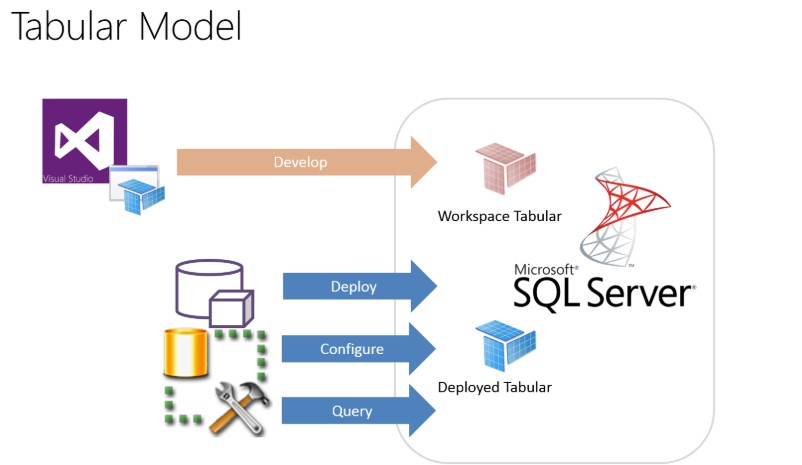
\includegraphics[width=12cm]{./Imagenes/img1} 
\end{center}


Sugerencias:
\begin{itemize}
	\item Primeramente, si ya se tiene una base de datos multidimensional, no se recomienda moverse a base de datos tabulares.
	\item El hardware requerido para un proyecto tabular es muy diferente al requerido por un proyecto multidimensional. Por la compresión de datos, requiere menos disco una modelo tabular, pero requiere mucha más memoria RAM porque todo lo usa en memoria. En general, se necesita un buen CPU y memoria.
	\item Los modelos tabulares consumen muchos recursos, por lo que se recomienda hacer pruebas del funcionamiento en un servidor de desarrollo y no en producción.
	\item Se puede tener un modelo tabular y uno multidimensional instalados en la misma máquina, pero no es recomendable hacerlo en producción.
\end{itemize}







\section{Ejemplo}
 
\section{Ventajas y Desventajas}

\subsection{Ventajas del Modelo Tabular}

\begin{itemize}
	\item Mucho más veloz en consultas.
	\item No requiere generar Aggregations (agregaciones) por lo que se simplifica el tiempo de procesamiento.
	\item Gracias al DAX (el lenguaje para acceder a los datos equivalente al MDX), tiene mayor flexibilidad para obtener información.
	\item Es intuitivo por lo que es mucho más rápido y fácil de entender e implementar.
	\item Se basa en modelos relacionales.
\end{itemize}

\subsection{Desventajas del Modelo Tabular}

\begin{itemize}
	\item Las particiones no se procesaban en paralelo si no secuencialmente, lo que hace que sea más lento el procesamiento.
	\item No se pueden usar multiples idiomas.
	\item Si son muchos datos tarda bastante en manejar configuraciones de diferentes particiones.
	\item El modelo tabular acapara demasiada memoria RAM y a su vez es dependiente de tal que afectará a otras aplicaciones.
\end{itemize}


\section{Diferencias}

\subsection{¿Qué modelo de datos utilizar? }

\begin{center}
	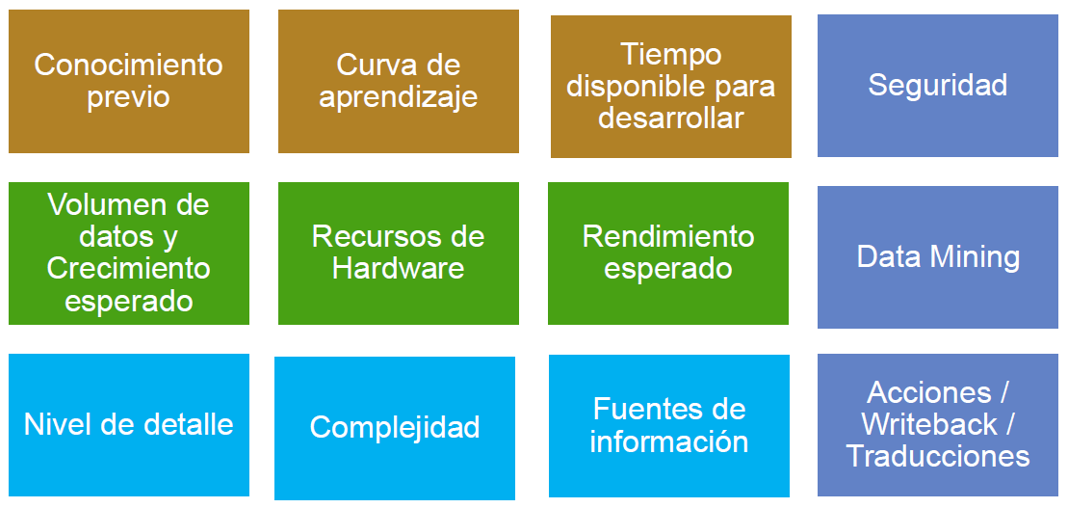
\includegraphics[width=12cm]{./Imagenes/dif0} 
\end{center}


\subsection{Diferencias del Modelo Multidimensional vs Modelo Tabular}

Diseño y Desarrollo\\
\begin{center}
	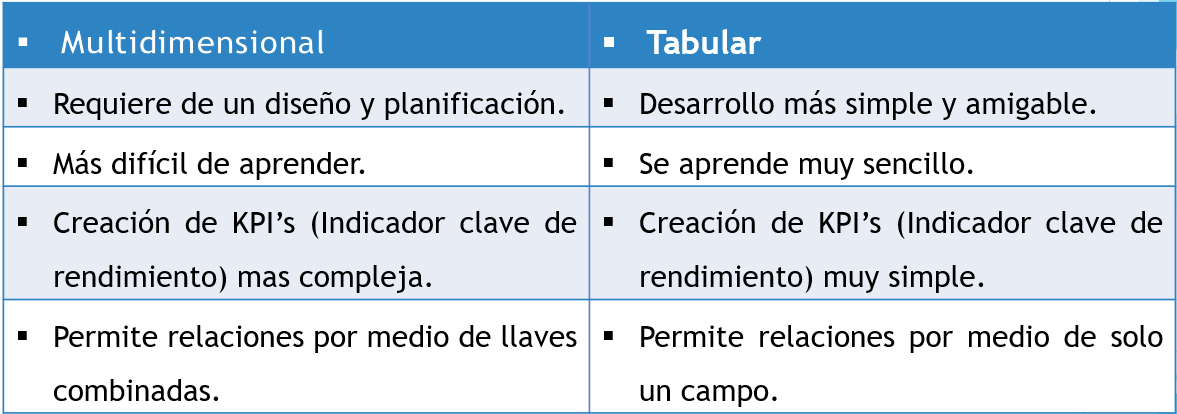
\includegraphics[width=12cm]{./Imagenes/dif1} 
\end{center}
\pagebreak
Desempeño y Escalabilidad\\
\begin{center}
	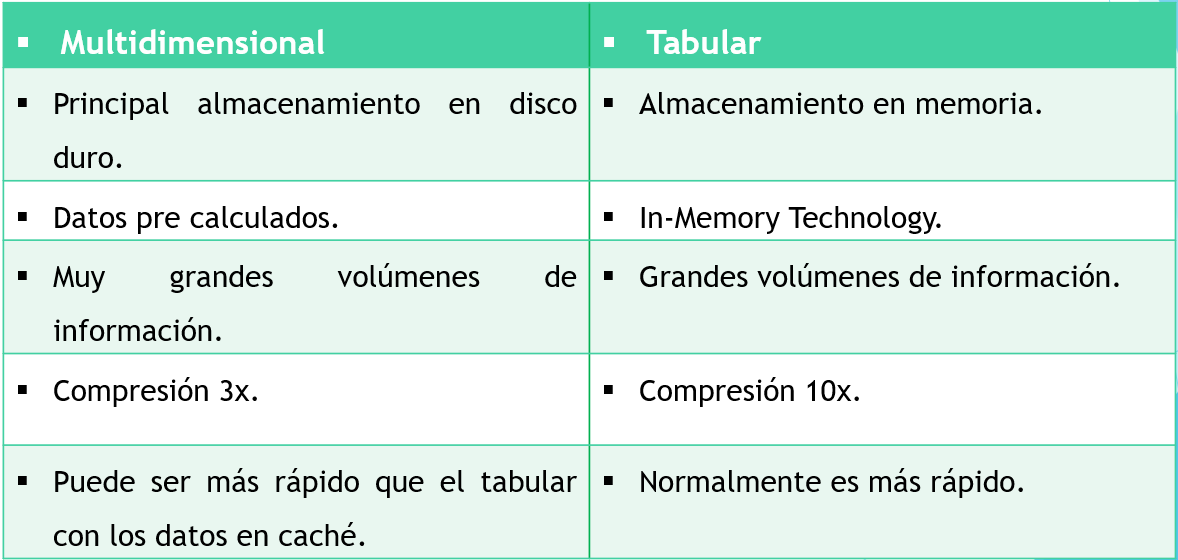
\includegraphics[width=12cm]{./Imagenes/dif2} 
\end{center}

\section{Conclusiones}


\begin{itemize}
	\item Como conclusión Microsoft le está apuntando al modelo Tabular, puede consultar las mejoras de la próxima versión SQL 2016. En SQL 2012 y 2014 el modelo Tabular es bueno para BI pequeños y medianos volúmenes, para altos volúmenes es preferible el modelo Multidimensional.
	\item Power View proporciona informes intuitivos adhoc para usuarios finales. 
	\item El modelo tabular no admite el procesamiento paralelo de particiones, lo que puede tener un impacto significativo en el tiempo de procesamiento.
	\item Microsoft realmente sabe cómo lidiar con los requisitos del usuario y sabe que faltaba un puente entre el modelo de base de datos de relaciones y el modelo MOLAP. 
	\item Al introducir el motor xVelocity en SSAS y el modelo tabular incorporado, Microsoft proporciona herramientas de acceso al usuario que proporcionan una mejor solución con buena velocidad y rendimiento. 
\end{itemize}

%%
	
	%%
	%\linenumbers
	
	%% main text

	
	\newpage
	
		%ESTILO
	%ARCHIVO .bib
	   \begin{thebibliography}{0}
              \bibitem{Juan} https://bib.irb.hr/datoteka/102195.t09r02.pdf 
                 \bibitem{Juan} https://www.sarjen.com/2016/03/15/what-are-the-pros-and-cons-of-tabular-model-over-multi-dimension-cube-and-relation-database/
                 \bibitem{Juan} https://www.element61.be/en/resource/choice-between-tabular-or-multidimensional-models-sql-server-analysis-services-2012
                  \bibitem{Jhordy} https://docs.microsoft.com/es-es/sql/analysis-services/comparing-tabular-and-multidimensional-solutions-ssas?view=sql-server-2017
 \bibitem{Jhordy} https://www.businessintelligence.info/definiciones/que-es-modelo-dimensional.html
                    \bibitem{Brandon} https://www.businessintelligence.info/definiciones/que-es-modelo-dimensional.html


         \end{thebibliography}
	
\end{document}

%%
%% End of file `elsarticle-template-1-num.tex'.
